\section{Introduction}
This section assumes familiarity with central biological dogma, as well as knowledge of basic concepts in Bioinformatics. Extensive background is provided in Appendix \ref{appendix:bio-background} that aims to accomidate readers of various backgrounds. The topics particularly relevant to this work are explained in the following sections. 

\section{Biological Background}
\label{appendix:bio-background}
\subsection{Central Dogma}
Amino acids, different properties
Proteins transcribed from genes - DNA that codes 

\subsection{Protein Folding}
Proteins are fundamentally polymers, or variable length chains of amino acid units joined together by covalent bonds.
The individual amino acids in a chain are referred to as residues. 
They all have two primary componets: a backbone consisting of a central carbon atom with two essential groups on oppsite sides: an \ce{-NH_2} amino gorup and a  \ce{-COOH} carboxyl group; and a variable side chain that is principally responsible for the physical and chemical properties of the residue.
\begin{figure}[ht] % replace with [H} if position is causing problems.
    \centering
    %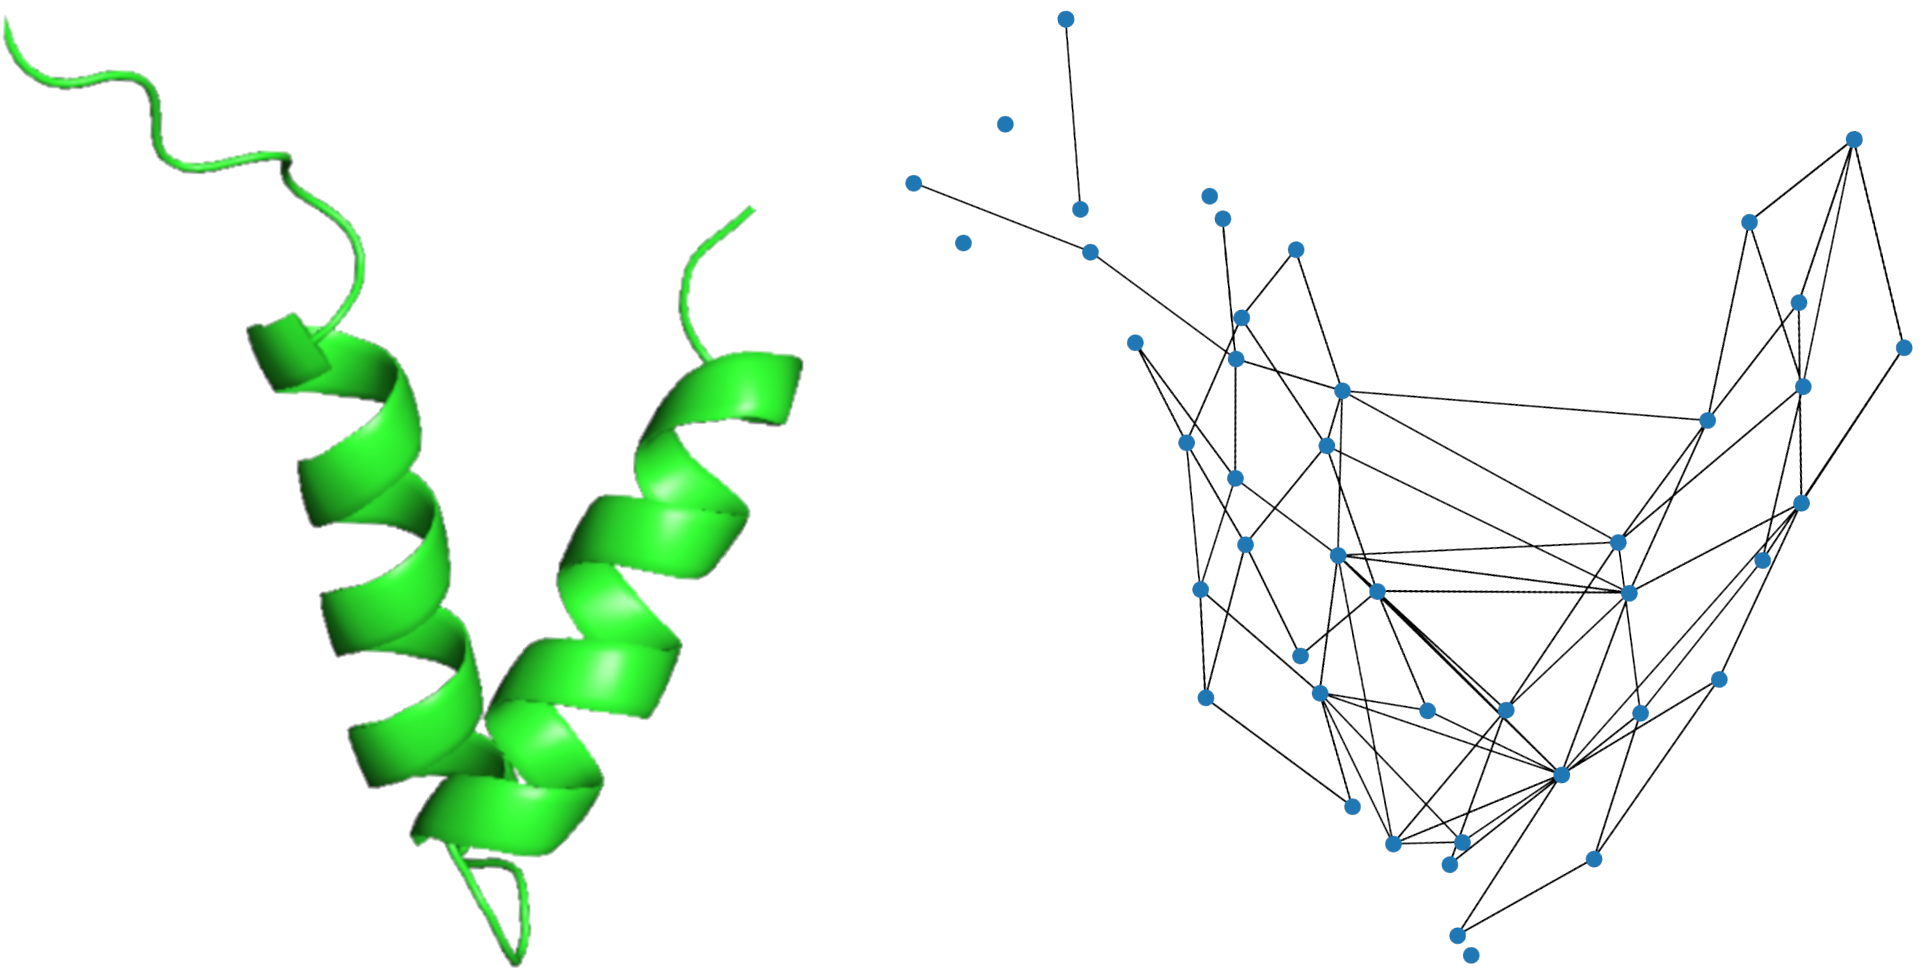
\includegraphics[width=0.5\textwidth]{fig/chain_to_RIN.png}
    \caption{Example of an amino acid structure.}
    \label{fig:AA-prop}
\end{figure}
Proteins are bonded together in a chain by forming peptide bonds --- a perticular kind of covalent bond where the amino group of one residue will bond to the carboxyl group of another. The sequence of the spesific residues in a protein chain is referred to as the \emph{primary structure} of a protein. 

There are 20 standard amino acids that primarly differ by their side chains. These side chains have varying polarity, charge, and size which effects the chemical and physical properties of the residue.

\begin{figure}[ht] % replace with [H} if position is causing problems.
    \centering
    %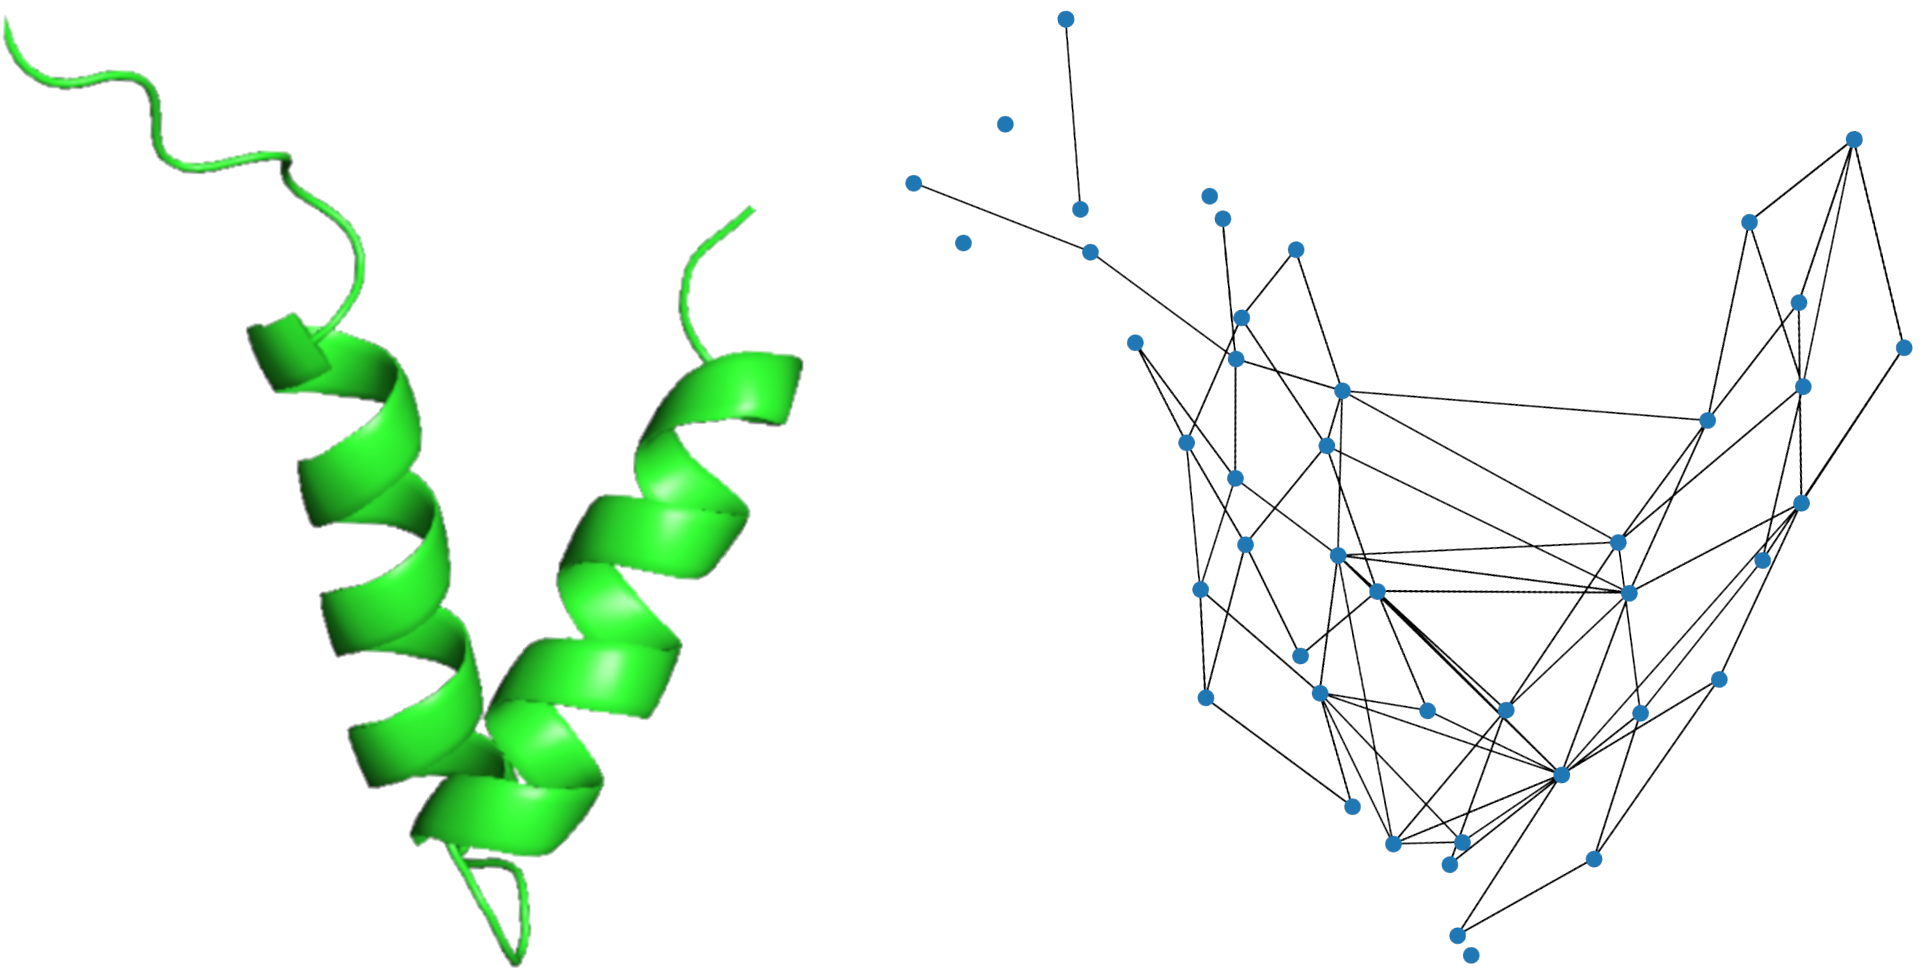
\includegraphics[width=0.5\textwidth]{fig/chain_to_RIN.png}
    \caption{The standard amino acid residues, groupped by properties.}
    \label{fig:AA-prop}
\end{figure}


Secondary Structure\\
Secondary structure of a protein refers to the most common local conformal patterns observed in the polypeptide chains constituting proteins. These patterns promote hydrogen bonding between atoms in the back bone of residues creating the beginnings of a structural scaffold.
The most common of these patterns are $\alpha$-helicies and $\beta$-strands. 
$\alpha$-helicies are right-handed spirals stabalized by hydrogen bonds formed between the oxygen of a carboxyl group and the hydrogen of an amide of another residue.

$\beta$-strands are linear chains of typically 5 to 10 amino acids. 
steatched out
alternating side chain orientation

$\beta$ sheets
can either be parallel or anit-parallel.
parallel slightly less stable
\begin{figure}[ht] % replace with [H} if position is causing problems.
    \centering
    %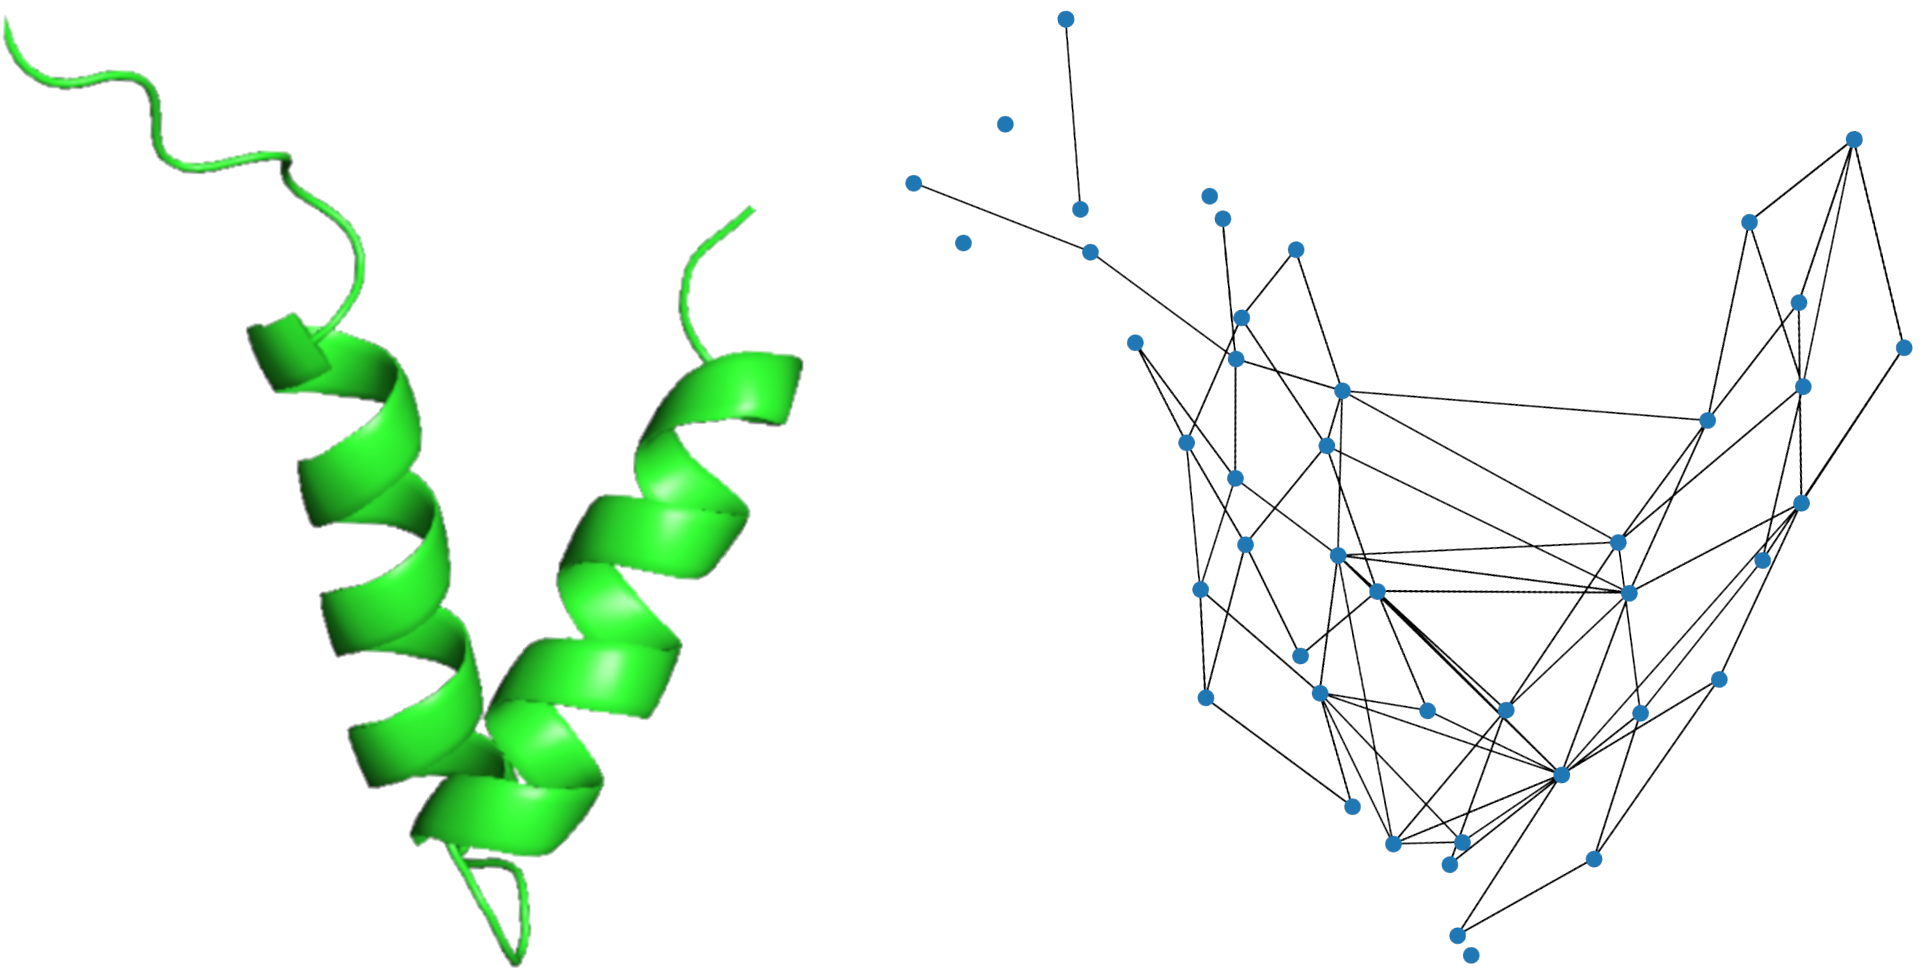
\includegraphics[width=0.5\textwidth]{fig/chain_to_RIN.png}
    \caption{The standard amino acid residues, groupped by properties.}
    \label{fig:secondary-struct}
\end{figure}

Tertiary Structure \& Protein folding\\
Tertiary structure refers to the oerall three dimensional conformation a protein adaps as it folds. This folding is dirven by a process influenced by the cellular enviroment and interactions between the different side chains of amino acids in the polypeptide sequence.
Quatrary Structure \& and protein complexes\\
Quatrary structure refers to the interaction between different polypeptide and other non peptide conpounds, or ligands to create protein complexes. 
These complexes 
It may be the case that a protein chain may occur in only one complex, where as some proteins may have a large network of interactiors with which it is observed in complex with.
We often refer to the spesificity of such interactions to describe the popensity of a protein to bind with only particular partners.

Complexes of multiple proteins are fromed primarially after a protein has folded and are they result of interactions between residues across the different protein chains.
To facilitate partner binding, proteins will have binding substrates with motifs, or notable amino acid sub-sequences, to facilitate a particular interaction. 
These regions or motifs are often critically important to the function of the structure 

Protein structure - function relationship
The final stucture or conformation of a protein is intrensiclly linked to the function of a protein.

\subsection{Homology}
It should be understood how several organisims may be evolutionarly related; from one common ancestor, mutuations are accumulated that may affect an individuals fitness, or the ability to thrive for a given enviroment.
These mutations are often neurtral, having not have much if any obsevable effect; however, mutations that alter fitness are most likely to be negatvie, but some mutations may confer a slight benifit to the individual and become selected. 
Accumulation of these mutations in a sub-population can lead to notably different traits and eventually speatiation. 
The discussion of these evolutionary relationships are well-defined at the orgranism level, but also do much to abstract away the low level on which changes occur. 
At the molecular level, proteins evolve through small changes that may lead to functional variations or the formation of evolutionarily related protein families. Mutations in the DNA of a gene can alter the protein sequence, while structural mutations like insertions, deletions, and inversions may lead to more significant changes. 
This process, known as \emph{molecular evolution}, descibes several different ways in which different protiens may be related. 

Homology is a general term that simply indicates that two or more proteis are related through a common protein ancestor. % find better word then member
%Orthologs
The common ancestor may be quite distant, even occuring befror a speciation event resulting to homologs in different species called \emph{orthologs}. These genes and the proteins for which they code often serve similar functions in the different species.
%paralogs
\emph{Paralogs} are genes within the same species that arise from duplication events of a sigle ancestral gene and result in, initially, two copies of gene and their protein product within the same species. They may diverge over time to adapt different structure or function, but often retain similar ones. Paralogs allow for diversity of similar proteins within a similar species and permit specilization in function.

Homologous proteins are often observed to functional and structural similarities, as mutations that radically impact the function of a protein are unlikely to confer an advantage. 
The theory of homology is frequently used to classifiy proteins into groups or faimilies usiving several different methods to form a taxonomy. 
%Could talk about pfam or cath if you want



Record providing direct evidence for two proteins being homologs most often cannot be established. Instead, homology is typically inferred through similarity between sequences. 
A common task is to find set or family of sequences related to a given query sequence through a \emph{homology search}. 
One such tool for performing these searches is BLAST, or Basic Local Alignment Search Tool, which identifies regions of high similarity between the given query and other known sequences. 
The match is visualize trough a pairwise alignment provided for each pair of query sequence - subject sequence match returned. 
There may be millions of sequences of a database, and inferring homology through a pairwise alignment can be a very difficult and computationally intensive problem. BLAST utility and prolific use can largely be attributed to its efficient implementation of its search algorithm, allowing for fast and accurate set of homologs using a heuristic search method. 
Details about different databases available for homology search and their content, as it pertains to this paper, is discussed in Section \ref{sec:DB-survey}.
% Why study homology

\subsection{Multiple Sequence Alignments}
Multiple Sequence Alignments (MSAs) function to align residues in a set of sequences. These could be sequences of arbitrary symbols. However, MSAs see extensive application aligning sequences of nucleotide sequences such as DNA or RNA, and protein sequences.
% I do not want to explain this
Nucleotide sequences use alphabets of A, T / U, C, G as stand-ins for nucleotide residues --- In DNA, these are adenine, guanine, cytosine, and thymine, respectively. Where in RNA sequences the same residues are observed with the exception of Uricil, denoted with a U, is seen where Thymine is not observed.
 % Protein residues and alphabet should be introduced in a previous subsection
 Amino acids in a protein sequence are identified in this context with a single letter code to designate each residue, as given in Figure~\ref{fig:AA-prop}.
There are many different tools for creating MSAs but all generally work by inserting gaps, designated by a `-', into the sequence. 
Creation of a MSA on a set of sequences typically assumes some form of homology, or evolutionary relationship between sequences in the set. 
A consequence of this assumption is that evolutionarly related sequences will exhibit some degree of similarity.
The use of MSAs allows for examine conserved sites or motifs in a family of sequences. When dealing with protein sequences, these conserved features often correspond to structurally or functionally important aspects of a protein.

\subsection{Structure Files}
%%% 3D structure files aid in the study of the 
The ability to resolve the structure of biomolucules has been transformative to biology as a whole---giving invaluable insigths to the functioning of processes on molecular level. Structural information is now a core aspect in a wide range of fields, providing a deeper understanding of molecular mechanisms that underpin life, from cellular processes to the development of novel therapeutics in areas such as medicine, biochemistry, and biotechnology.

%%% Experimental methods
Protein strctures are determined experimentally using methods such as X-ray chrystallography, nuclear magnetic resinance (NMR) spectroscopy, or cryo-electron microscopy (cryo-EM). 
X-ray chrystallography requires a purifed protein sample to be chrystallized. Passing a high-power X-ray beam through the chrystal results in the creation of a diffraction pattern that is used to determine the 3-D structure of a protein through numerical methods like inverse Fourier Transform. This results in high quality position information, with enough spacial resolution to accurately determine the position of individual moldecules. The need for a high purity chrystal sample, however, can pose a significant limitation, as proteins with dynamic conformation such as intrensically disordered proteins (IDP), or highly hydrophobic proteins like trans-membrane proteins (TMP) can be difficult to chrystallize, resulting in bias in the structural information avaible using this method \cite{PDB-bias}. \todo{An image could be inserted here if filler is needed.}
%MNR
NMR explotis the magnetic properties of atoms nuclei to resolve their position. NMR works by applying a magnetic field to a protein sample and detecting the energy released as the atomic nuclei return to their original states, which helps determine the distances between atoms. NMR has the benifit of being able to study proteins in solution, allowing for observation in conditions that may more similarly resemble their normal biological conditions. Furthermore, the technique is particularly useful for observing the conformal dynamics of flexiable proteins. 
%Cyro-EM
Cryo-EM involves rapidly freezing protein samples in a thin layer of ice to preserve their native structure, then using  electron microscopy to capture high-resolution images of the sample. Thousands of these 2D images are collected and combined using computational techniques to reconstruct a 3D model of the protein. This method is particularly effective for studying large molecular complexes and proteins that are difficult to crystallize.

% Alpahafold aside
Accessiability to strucutural information obrained by such experiments has been revolutionary for the feild of Bioinformatics. This is facilitated by standardized file formats for structural data and databases to catalogue and facilitate access to information. The Protein Databank (PDB) is the foremost database for structural data, offering a comprehensive resource for published experimental structures. 
% more about the database
The avaibility of experimental structural data enabled the training of models such as RosettaFold and Alphafold, which are both machine learning models capable of creating high accuracy predictions of protein structure given an amino acid sequence. Predictions for AlphaFold2 are catalogued in a database and publically avaible. More information about AlphaFold and its structure database are avaible in.\todo{link ref}

As previously mentioned, strucute files availible in such databases are stabdarduzed to aid in machine and human readability. One of the notable early efforts to do this was with the PDB file format, wich still enjoys prevelence, but is in the process of being displaced by the more recent PDBx/mmCIF format (eXtended PDB/Macromolecular Crystallographic Information File). In this work we focus on the mmCIF file format, commonly refered to as just CIF, as HomologyRing is made to work exclusively with this file format.
%%% Introduce CIF, give schema and data higharchy.
The CIF format uses dictionary-based schema allowing for notable extensibility, allowing for effective storage of many different data types. 
A great deal of metadata are included in these structure files; giving biological context to the structure by giving experimental and author information, indicating what genes and organisim a protein chain was transcribed from, pH information and other physical information, what experimental methods were used, mutation information, amoung others. 

%%% Organization of CIFs
Perhaps the most important section of a CIF details the position and identity of atoms in the structure. This is detailed, internally, in the \texttt{\_atom\_site} category, and adhears to a heigharical structure wich is important for the both the biological asseblies of protein complexes and working with said structures in a structural Bionformatics context. In a CIF protein structure, individual atoms will have a set of identifing and associated information like a numerical identifier, symbol corresponding the atoms element, 3-D coordinates, compositon ID, a sequence ID, and chain identifiers. 
The composition ID, sequence ID, and chain identiefiers are both used to assign atom membership to groups within the CIF data higharchy. This higharchy formalizes biologically relevant concepts used to describe polymers like DNA and proteins into a well-defined data structure with several levels: atom, residue, entity, chian (molecule), and structure (complex). Atoms belong to residues in polymers. In proteins these are the individual peptides which are identified within the \texttt{\_atom\_site} section of a CIF by their composition id with their abbreviations like `ALA' for Alinine, `CYS' for Cystine, or `PRO' for Proline, for example, with a similar system for the nucleic acids. Residues are assigned a numerical index, or sequence ID, with in their polymer chain

Additionally, some atoms not belong to the a macromolecule -- polymers like RNA, DNA, or proteins which are most frequently the primary subjects of study in CIFs. such atoms are reffered to as `hetroganous atoms' or \texttt{HETATM} for short. These capture metal ions, water molecules, or ligands, that are biologically relevant to and captured along side the experimental structure. Ligands are molecules that bind to a larger molecule to form a complex and play essential roles in biological processes.

%%% TODO 10/31
% Finish explaing residues, chains, and entities
% reference image
% integrate already written content
% mess around with centrality

\begin{figure}[ht] % replace with [H} if position is causing problems.
    \centering
    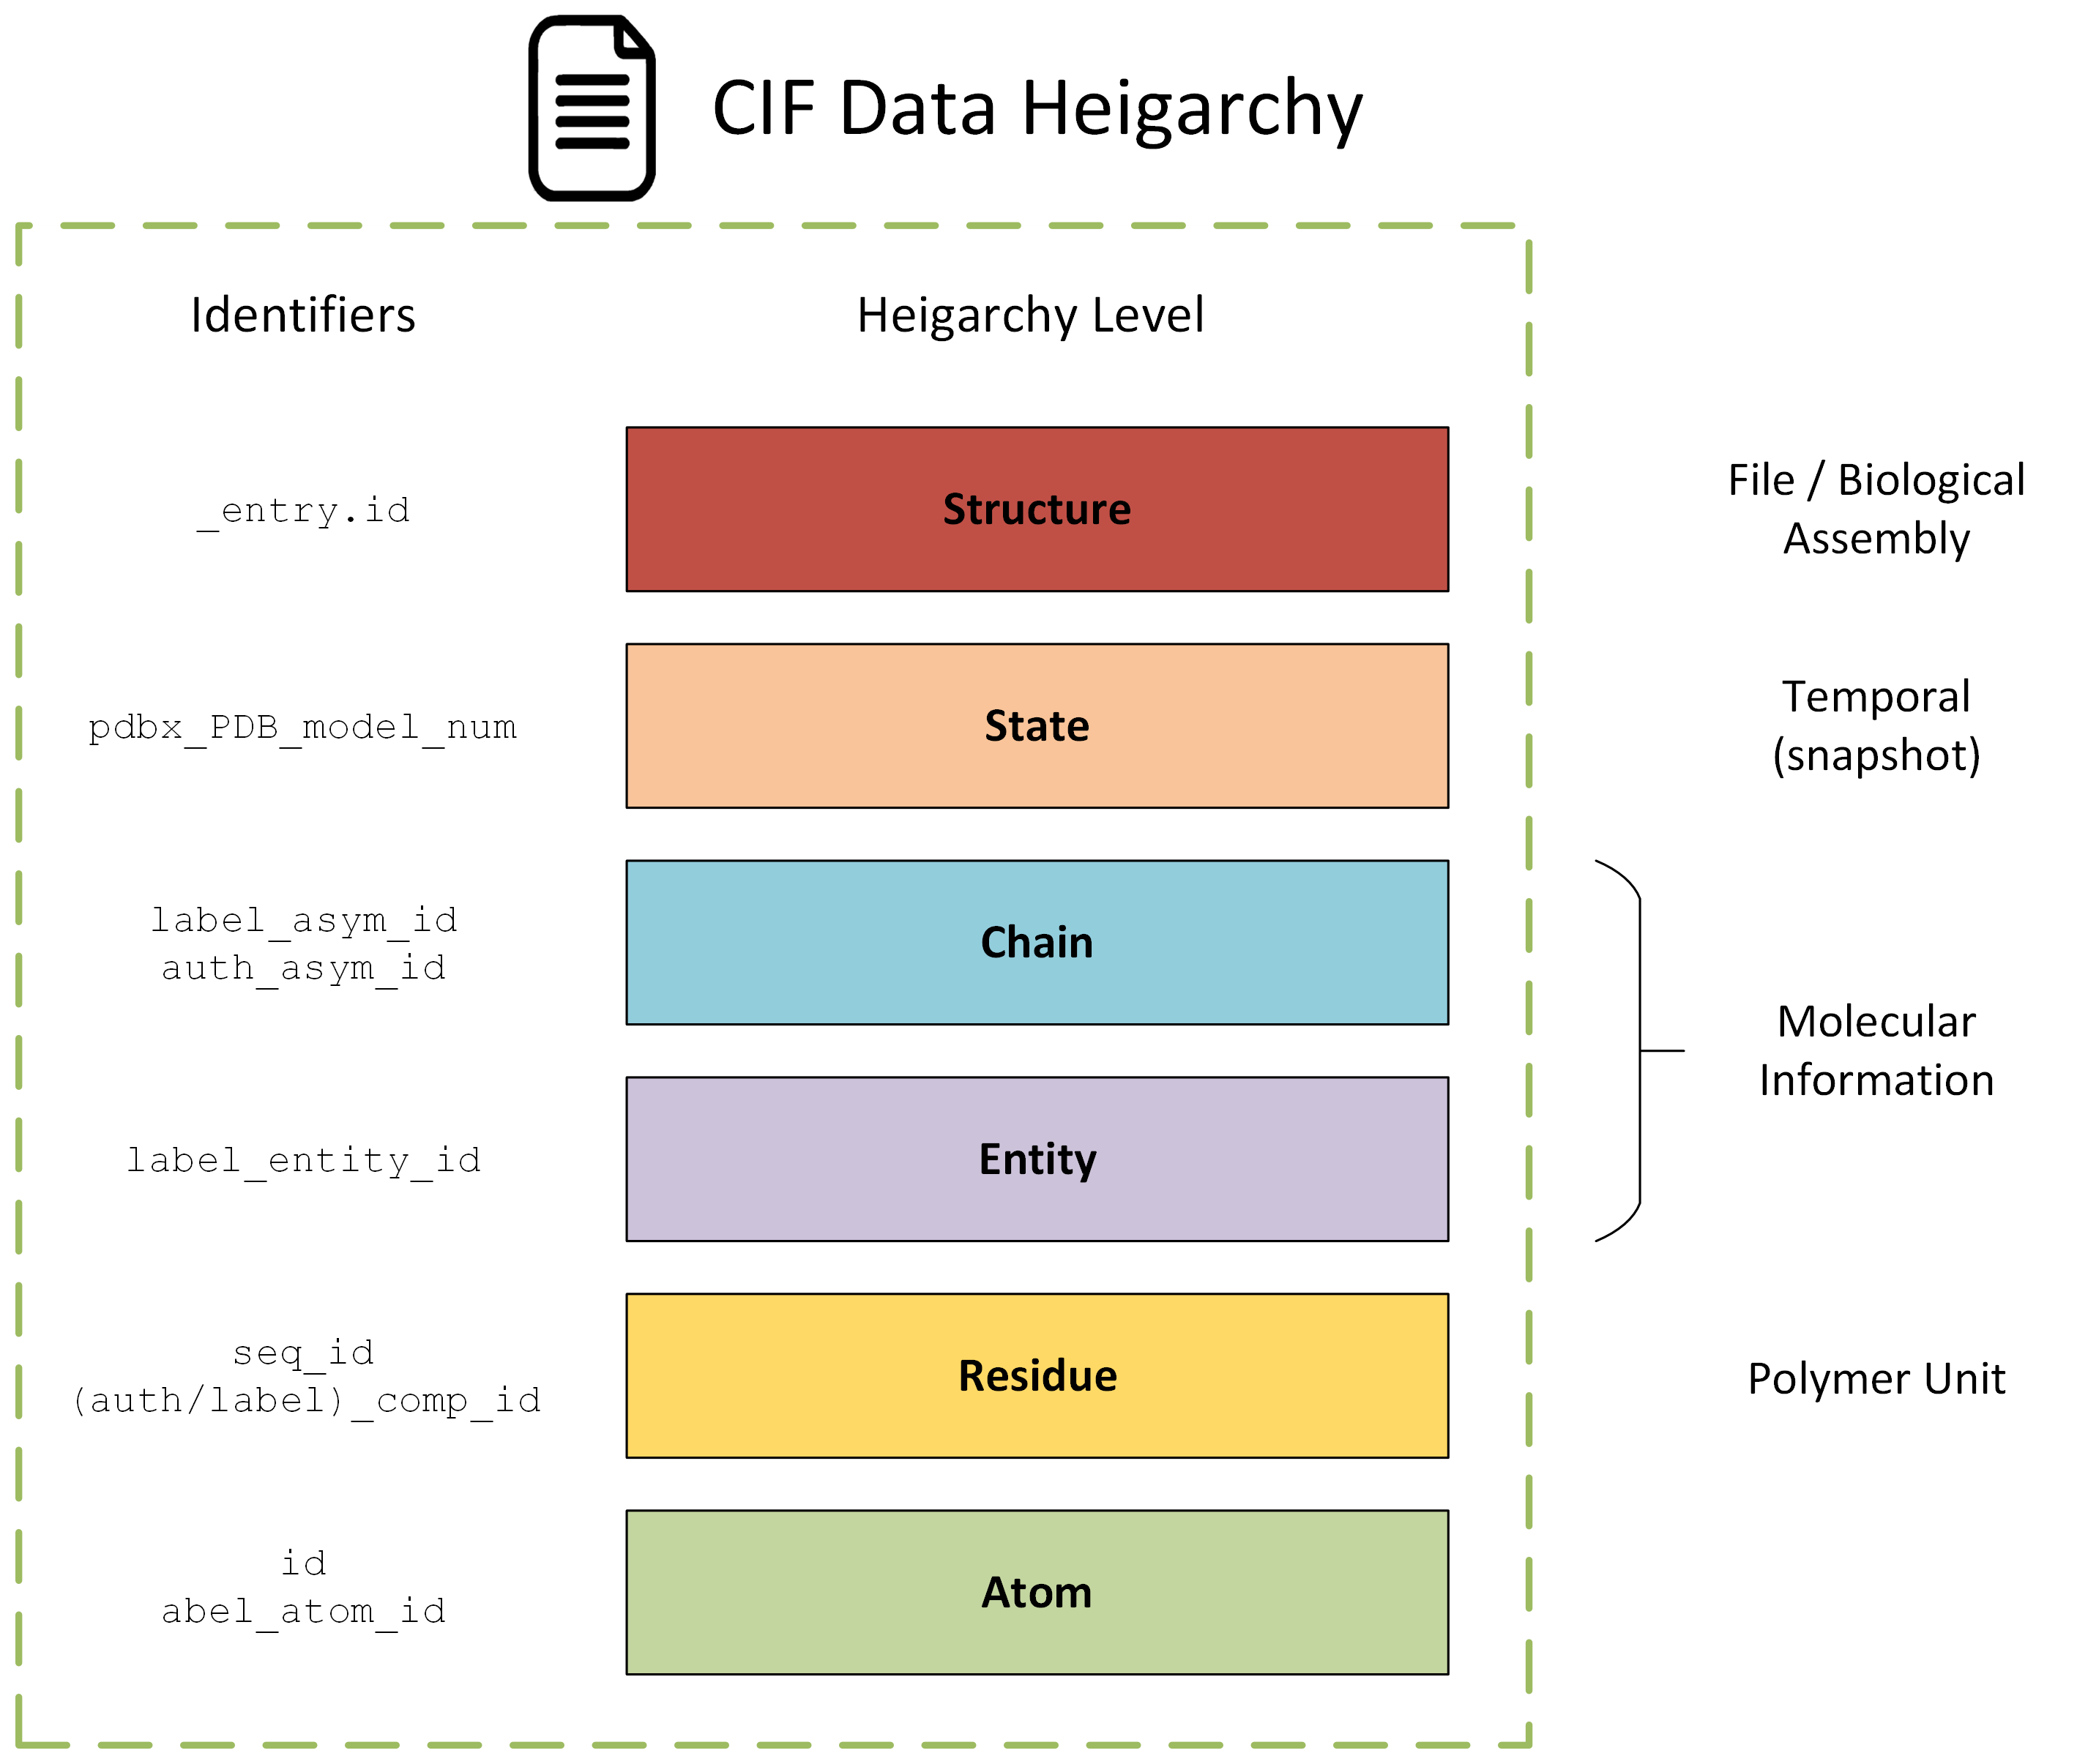
\includegraphics[width=0.5\textwidth]{fig/CIF_data_schema.png}
    \caption{Diagram displaying the various levels of the data organization of structural information in the CIF format.}
    \label{fig:CIF-heigharcy}
\end{figure}

CIFs are supported by a host of software common for structural analysis. Structural viewers like PyMol and Chimera  allow for visual interpretation of a structure which is immediately quite useful for gaining an intuition for the conformation of a protein. However, this is still not without limitations: structuers are often large and quite intricate, requiring the use of cartoon representations of chains to limit the amount of visual information presented to a user. Furthermore, intrepiting functional consequence of strucutres often take a lot of time and biological expertiese. This problem is aided by anotations present in structure databases, as well as many different software tools for performing spesific analysis such structures, something we do as well in this work. % bad wording
HomologyRing supports the use of either PDB or AlphaFold Database for homology search. The choice of which to use will depend on the motivation of their analysis. Differences between these databases and the benifitis of each source is discussed in Section \ref{sec:DB-survey}
.%%% CIF file higharchy
Each structure of a family will contain atleast one entity. These entities may be polymers such as DNA, RNA, or polypeptides; or non-polymer entities like water, or other compounds like co-factors. Each entity is given its own numeric internal identifier within a cif file, which are grouped into chains, identified by a character code. 
%%% Blurb on why HomologyRing is based
Structure files of this form can be quite large, commonly 10s of megabytes, and repositories of structures rapidly become very large.
The PDB contains on the order of 300 GB of structural data and the AlphaFold Database is estimated to be between 20--30 TB. 
This makes performaing analysis at scale of such files, as needed for homology studies potentially quite storage intensive.

The CIF format does has the benefit of being both human readable in text form and machine parceable. However, information about the geometry of the structure is given by the position of discrete atoms. This makes extracting biologically relevant information that one may want from 
Both of these factors can make inferring relevant information from structures at scale quite difficult. HomolgyRing provides a method for encoding structural information for a family of proteins into a network. The process of which is outlined in Section \ref{sec:hRIN}.

\section{Residue Interaction Networks}
At the very basic level, protein chains are polymers of amino acid residues bound together by covalent bonds. As a chain folds, it is \emph{non-covalent} interactions between residues that are principally responsible for the secondary and tertiary structure (conformation) of the protein. These non-covalent interactions could be a verity of different forces and are the result of the different chemical and physical properties of the 20 different base amino acids and their arrangement in the peptide sequence that constitutes the protein chain. 
Examples of interactions commonly observed witnin proteins include Van Der Walls forces and hydrogen bonding. Other interactions are observed less frequently and exibihit high specificity with respect to amino acid participants, like Ionic bonds or $\pi-\pi$ interactions and several others. 
%Need to mention the structure component again
Furthermore, the structure of a protein is intrensically tied to it's function within its biological context. % Why are you mentioning this here
With this in mind, there's a lot of information that can be gathered from knowledge of these non-covalent interactions. 
Researchers may very easily interpret the structural or functional significance of an interaction, but methods concerning non-covalent interactions can be applied to a problem long troubling structural bioinformatics: The amount of available structural information has been growing at a near exponential rate. % citation
Both experimental structures available through the PDB and high accuracy predictions given by AlphaFold2 are commonly available in PDB or mmCIF file formats. These files are large---containing 3D atom data, chemical information, and a host of metadata. Parsing, and algorithmically extracting functionally relevant information algorithmically proves to be an arduous task in many contexts. 
One approach to addressing this problem has garnered much attention: The construction of Residue Interaction Networks (RIN) use information of non-covalent interactions to create a simplified representation of a protein structure.
There are many variants of the idea. However, they are generally defined for a protein structure to be a mathematical graph, or network, denoted $G = (N, E)$ where $N$ is a set of nodes identifying amino acid residues or various compounds in a structure and $E$ is taken the set of non-covalent interactions observed in the given structure.
An example of such a network is shown in figure \ref{fig:ex-prot-RIN}. RINs can be seen to provide a simplified means of capturing the topology of a protein structure, and has seen notable attention for its various applications:
%Applications of RIN
Binding, protein engineering... 
Training data of machine learning methods like graph neural networks (GNN). 
Historical methods like Convolutional neural networks (CNN) on distance matricies discard physicochemical information and may be considerable larger than analogous representation of the same structure with a RIN. 

\begin{figure}[ht] % replace with [H} if position is causing problems.
    \centering
    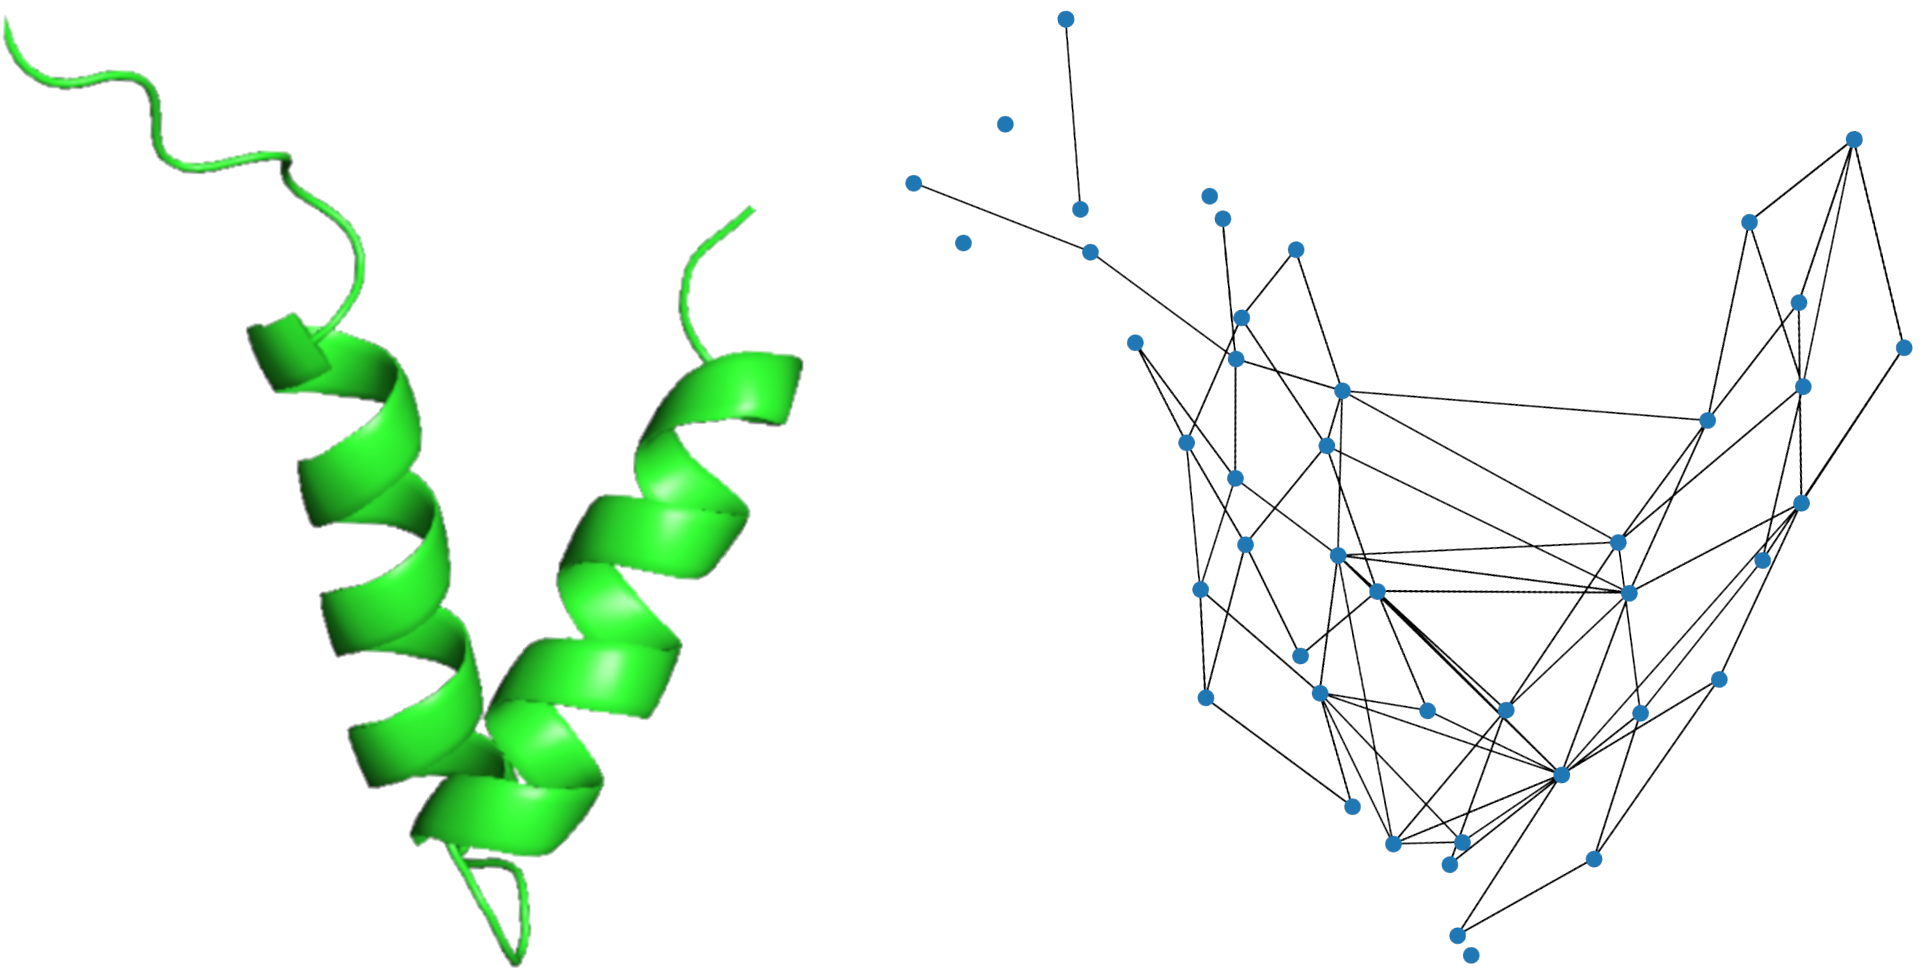
\includegraphics[width=0.5\textwidth]{fig/chain_to_RIN.png}
    \caption{Example of a basic RIN for generated for a protein chain.}
    \label{fig:ex-prot-RIN}
\end{figure}

\todo{If you are going to weight edges with prob for ensembles, it should go here.}

\subsection{Residue Interaction Network Generator - RING}
There are many available tools capable of generating RINs, each with a slightly different interpretation of the object. In this work, such networks are created using Residue Interaction Network Generator - RING. Notable for its ability to handle all ligands and modified residues in the PDB, it is regarded for accurately and deterministically predicting non-covalent interactions within structure files. It is worth noting that the output of RING is a multi-Graph. Differing from the typical mathematical notion of a graph, it permits multiple edges between a given pair of nodes (see Figure \ref{fig:ex-RING}). These different edges correspond to the different non-covalent interactions predicted by RING. The list of interactions predicted by RING comprising the possible edge types in the resulting RINs are described in Appendix \ref{appendix:RING-inter}. Furthermore, we will refer to the various interaction types by their internal RING identifiers throughout this text for the sake of brevity and clarity (e.g. \texttt{HBOND} for hydrogen bonding and \texttt{IONIC} for salt bridges).

\begin{figure}[ht] % replace with [H} if position is causing problems.
    \centering
    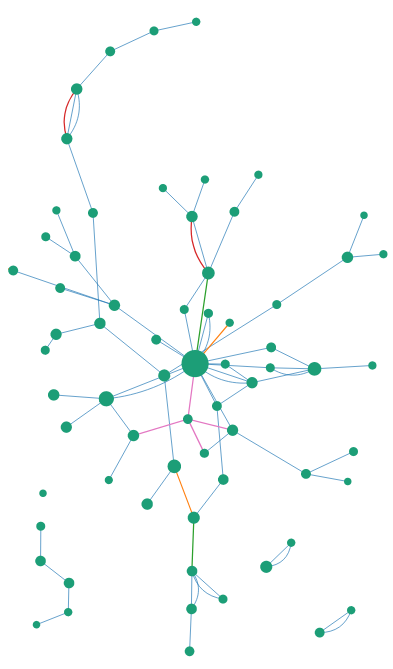
\includegraphics[angle=90, width=0.5\textwidth, height=0.3\textheight, keepaspectratio]{fig/ex_RING.png}
    \caption{Example of a RIN multi-graph visualization created with RING. As typical with RINs, nodes correspond to amino acid residues in a given protein structure. Edges correspond are non-peptide interactions or bonds between residues. Where edges of many interactions are types are permitted between a pair of nodes.}
    \label{fig:ex-RING}
\end{figure}

\section{Appendix: RING - Predicted Interactions} 
\label{appendix:RING-inter}
RING predicts and classifies various types of molecular interactions based on deterministic factors such as geometric orientation, distance, and the chemical nature of the compounds involved. These interactions differ significantly in their chemical and physical properties, including strength and specificity, which in turn influence the likelihood of different amino acids forming specific bonds. Understanding these variations is essential for interpreting the structural consequences and functional roles of these interactions on the atomic and protein level as well as in the context of RINs and hRINs. This section will define and provide context for all interaction types classified by RING, enabling a better understanding of their role in protein structure and function.

\subsection{Van Der Waals Forces - \texttt{VDW}}
Van der Waals forces are relatively weak non-covalent interactions between molecules or atoms. In fact, they they are considered one of the weakest interactions observed at the atomic level. 
VDW forces arise from temporary shifts in electron density induced by the proximity of other molecules or atoms. These shifts occur because of fluctuations in the electron cloud, leading to temporary dipoles. As a result, Van der Waals forces can be either attractive or repulsive.
At very small distances, the repulsive forces dominate due to the proximity of electron clouds, while at larger distances, the attractive forces generated by induced dipoles become prominent. This balance creates a stable equilibrium distance, which plays a key role in maintaining weak but widespread interactions.
%With this in mind, there are three different types of Van Der Waals forces: \todo{I don't think most biologists/users care}
%\begin{itemize} 
%	\item \textbf{London Dispersion Forces}: 
%	\item \textbf{Dipole-Dipole Interactions}: 
%	\item \textbf{Dipole--Induced Dipole interaction}
%\end{itemize}

In proteins, the have prolific presence, as they arise from virtually all residues that would would considered to be in contact. Though individually, a VDW interaction represents a small force, their accumulative effect over large substrates allows them to play a significant role in tertiary and quatrnary structure. 
They are of notable interpretation in the context of RINs, where a great of protein topology is captured by VDW forces, as they can be used as an indicator of residue proximity. However, in practice, they often prove difficult to use in this way. Working with structure or topology information directly can be a complex task. Furthermore, they provide a great deal of data, with a residue often experiencing VDW interactions with many other residues. This surplus of data often hinders the extraction of useful information. 
In a protein family, the VDW interactions tend to be poorly conserved, and given their abundance, it is difficult to prescribe functional importance to a subset of VDW interactions in a family. For this reason, we often choose to filter them in our analysis to highlight the effect of more interactions with higher specificity.

\subsection{Hydrogen Bonds - \texttt{HBOND}}
Hydrogen bonds are most prolific non-covalent interactions second to VDW forces. They are most commonly observed 
in their role of maintaining secondary structure components: $\alpha$-helices and $\beta$-sheets. 
Hydrogen bonding is most prevalent in amino acids with polar side chains, where electronegative atoms like oxygen, nitrogen, and sulfur

However, they are also commonly observed among tertiary interactions, stabilizing the overall conformation of a chain, and quaternary interactions to form complexes. Hydrogen bonding is additionally of notable importance for protein-nucleotide interactions \cite{}. 
Residues most commonly forming these interactions are serine, threonine, asparagine, and glutamine. \cite{}

Information of hydrogen bonding in protein families provides is quite useful, despite their prolific nature. 
it is commonly observed that the preservation of local conformation of functional sites will be critical, even in a family of distantly related proteins. Conservation of hydrogen bonding corresponds to regions of high sequences conservation for interactions of short distance
\subsection{Ionic Bonds - \texttt{IONIC}}
Ionic bonds occur at the atomic level when an electron is transferred from one atom to another. The resulting atoms, having transferred an electron, become ionized hand have and each have a net charge. The donor will exhibit a positive charge, while the recipient becomes negatively charged. This difference in charge, creats a strong electrostatic attraction, bonding the two atoms. 
In proteins, ionic bonds are often referred to as \emph{salt bridges}, and their formation generally require the presence of amino acids with charged side chains. These include: lysine, arginine, and histidine with positive charge; and asperic and glutamic acid have negatively charged side chains.
This creates a loose relationship between conservation of these residues in a sequence and the conservation of ionic bonds they may participate in in a structure. % Possibly remove. At very least reword.
The ability of the charged amino acids to participate in ionic bonds is pH dependent. This allows some proteins to adapt variable conformations in response to cellular environment; this is one possible functional interpretation of an ionic bond with in a protein.

\subsection{$\pi-\pi$ Stacking - \texttt{PIPISTACK}}
$\pi$-$\pi$ stacks are spesifc interactions between pairs of aromatic rings; or stable, planar, ring-shaped molecular structures with alternating single and double bonds present in some amino acid side chains.
In proteins, such amino acids with requierd for the interaction are: phenylalanine, tyrosine, histidine, and tryptophan. 
These aromatic rings have decentralized $\pi$-electrons, to which the interaction owes its name. 
These electrons have distributions not centralized around a single atom, as typically the case, but rather the electrons may exist in a shared annular cloud around the aromatic ring.
These perculiar electron distributions permit specialized interactions: either with other aromatic rings to form a $\pi-\pi$ interactions, or other compounds, as seen later.

$\pi-\pi$ interactions may have one of two possible configurations of the participating aromatic rings: 
\begin{itemize}
    \item \textbf{Face-to-face}: where the rings are stacked directly on top of each other with a slight offset.
    \item \textbf{Edge-to-face}: where the rings are oriented perpendicularly, with the edge of one ring pointing toward the center of the other.
\end{itemize}
In both cases, the interaction of the $\pi$-systems creates an attractive force that stabilizes the residues relative positions.

These interactions tend to be quite specific and relatively well preserved.
Often serve to stabilize tertiary and quatrary structure. Given this role they are quite useful for characterizing a families topology.

\subsection{$\pi$-cation Bond - \texttt{PICATION}} \todo{both pi cation and pi pi stacking have noteworthy roles in binding with pi systems in ligands}
Similar to $\pi$-$\pi$ interactions, $\pi$-cation interactions require the particular electron distribution of a $\pi$ system seen in an aromatic ring. However,

Donor cations can belong to another residue with a positively charged side chain, allowing the interaction to play a notable role in tertiary and quatrary structure stabalization.
Beyond intra or inter--chain interactions, $\pi$-cation interactions or often important for ligand binding and in enzyme active sites; where aromatic residues can be used to locate cations and stabalize interactions.

in these interactions the system is to considered to donate a $\pi$ electron to the cation, which becomes a $\pi$-acceptor.

\subsection{$\pi$-hydrogen Bond - \texttt{PIHBOND}}
Similar in action to both $\pi$-cation bonds and typical hydrogen bonding, $\pi$-hydrogen bonds are stabalizng interactions where a positively charge hydrogen bond donor, such as a polar \ce{-OH} or \ce{-NH} group, interacts with the electron rich $\pi$ system of an aromatic rings, present if several amino acid side chains.
$\pi$ hydrogen bonds are weaker and far less common than both $\pi$-cation and $\pi$-$\pi$ stack interactions. As a result they tend be less frequently important for the structure and function of a protein, and they are observed to often not constitue a significant part or residue interaction networks. However, there are notable exampels where they perform a significant role, such as in DNA binding proteins such as transcription factors and aromatic rich enzyme active sites. \todo{this is interesting. see if you can expand on the DNA binding}

\subsection{Halogen Bonds - \texttt{HALOGEN}}
Halogen bonding is a non-covalent interaction involving a halogen atom (such as fluorine, chlorine, bromine, or iodine) and an electron-rich atom or group (such as oxygen, nitrogen, or sulfur) acting as an electron donor. Although halogens are typically considered electronegative, when they participate in covalent bonds, they exhibit a region of positive electrostatic potential called the $\sigma$-hole on the side opposite to the bond. This $\sigma$-hole allows the halogen to act as an electron acceptor, facilitating the formation of a halogen bond with an electron donor. 
In proteins, 

\subsection{Disulphide Bonds - \texttt{SSBOND}}
Disulphide bonds, also called disulphide bridges, are uniqe in this list of interactions as they are covalent bonds; and the amino acid cystine is also unique for its sulpfur containing \ce{-SH} thiol group in its side chain, need for the formation of disulfide bonds.
The formation of the sulfur bridge reqires an oxidation reaction where the hydrogen is displaced, and results in a \ce{S-S} interaction that is considerably stronger and more sable than many of the other inter-residue interactions witin a protien. That said, they are reversable under reducing conditions, allowing for dynamic protein conformations that are responsive to certain cellular conditions. The strength of the covalent bond is durable in harsh extracellular conditions, and is often seen stabilizing structure in such enviroments. 
These bonds are generally seen to have notable separation in a protein chain or present in typically well preserved inter-chain interactions. \todo{cite and more details}
This gives cystine a clear role in contributing to tertiary and quaternary structure of proteins. 
Due to the unique nature of cystine and disulfide bridges, cystines are frequently well preserved at the sequence level within a protein family and so too are associated disulfide interactions.
Cystine is notable for participating in other interactions such as metal coordination, or enzymatic activity, but where it participates in in disulfide bridges, tend to represent highly conserved sites within a protein family.

\subsection{Metal Coordination - \texttt{METAL\_ION}}
Involves the interaction of a metallic cation.
Metal Coordination bonds can be covalent, where they are also called dative bonds, or non-covalent.
Even non-covalent metal coordination interactions tend to be high strength interactions.
Coordinate Covalent bonds are particular because a pair of electrons involved from the bond are donated by a single atom (often nitrogen, oxygen, or sulfur) and paired with an electron-deficient acceptor. 
Since the donor contributes a pair of electrons, the most common acceptors for this type of interaction are \ce{Zn^{2+}}, \ce{Fe^{2+}}, and \ce{Cu^{2+}}.

Metals in proteins have a key roll in electron transfer processes, allowing proteins to facilitate redox reactions. 
Finally, centrally coordinated metals often of great strucural significance, as the strong coordination interactions work to stabalise the conformation of a protein as is the case with zinc finger proteins where cystine and histidine bound to a \ce{Zn^{2+}} ion gives the structure its iconic shape, enabling DNA and RNA binding. 

Metal coordination, then, most often represent critical components of a proteins structure or function and consequently are frequently well perserved in families. However, experimental and procedral variation in structure creation can make there presence inconsistent in some senerios. Notably, AlphaFold2 does not predict the presence of metals, or other ligands, so will not be represented in predicted structures.  

\section{Appendix: Installation and Dependencies}
The code repository can is available from the BiocomputingUP GitHub: \\
\href{https://github.com/BioComputingUP/ring-homology-pipeline}{https://github.com/BioComputingUP/ring-homology-pipeline}\\
Execution of the pipeline has a set of commandline programs be installed and correctly added to \texttt{PATH}. 

\vspace{0.5cm}

\begin{tabular}{l l}
\textbf{BLAST Command Line} & \url{https://www.ncbi.nlm.nih.gov/books/NBK279690/} \\
\textbf{Clustal$\Omega$} & \url{http://www.clustal.org/omega/} \\
\textbf{RING standalone} & \url{https://ring.biocomputingup.it/} \\
\end{tabular}
\vspace{0.5cm}

Note that ring4.0 command line is needed for use of \texttt{use\_label\_asym\_id} argument when building a hRIN. 
Additionally, commandline BLAST requires copies of databases be built and installed locally inorder to perform a homology search. The two that we display in this paper and are likely to be of particular interest to a user is `\texttt{swissprot}' and `\texttt{pdb}' which may be downloaded from the BLAST FTP server. Files, typically in FASTA format must be built into blast databases using the BLAST commandline tool and placed into the \texttt{blast\_db} directory. 
The user may alternatively create their own blast database with the same method, however, it should be noted that the resulting database may have a different schema and the config file: \texttt{config.json} may have to be modified to allow for successful parsing. \todo{Trying to deprecate this, if possible}
Specifying that the homology search should be performed remotely with the \texttt{remote\_BLAST} argument can avoid the need for a local blast installation. However, it should be noted that the search usually takes much longer on NCBI servers.